% Style for a MSc paper at Warsaw School of Economics
% Michał Ramsza
% Friday, December 14, 2012

% --- document class and other global stuff ---------------------------
\documentclass[polish, twoside, 12pt, a4paper]{article}

% --- packages --------------------------------------------------------
\usepackage{textcomp}
\usepackage{times}
\usepackage{amsmath}
\usepackage{amsfonts}
\usepackage{amssymb}
\usepackage{amsthm}
\usepackage[T1]{fontenc}
\usepackage[utf8]{inputenc}
\usepackage{graphicx}
\usepackage{xcolor}
\usepackage{enumitem}
\usepackage[polish]{babel}
\usepackage[centering, left=3.5cm, right=2.5cm, textheight=24cm]{geometry}
\usepackage{tikz}
\usepackage{pgf-umlcd}

% --- tikz-----------------------------------------------------------------

\usetikzlibrary{shapes.callouts}

\tikzset{
  level/.style   = { ultra thick, blue },
  connect/.style = { dashed, gray },
  connect_k/.style = { dashed, red },
  notice/.style  = { draw, rectangle callout, callout relative pointer={#1} },
  label/.style   = { text width=2cm }
}


% --- packages for citations ------------------------------------------
\usepackage{natbib}
\AtBeginDocument{\renewcommand{\harvardand}{i}}

% --- package for automatic insertion of R code -----------------------
\usepackage{listings}
\lstset{language=R,%
   numbers=left,%
   tabsize=3,%
   numberstyle=\footnotesize,%
   basicstyle=\ttfamily \footnotesize \color{black},%
   escapeinside={(*@}{@*)}}

% --- support for links -----------------------------------------------	
\usepackage{url}
\usepackage{hyperref}
\hypersetup{colorlinks=true,
            linkcolor=black,
            citecolor=darkgray,
            urlcolor=darkgray,
            pagecolor=darkgray}

% --- support for large tables and other stuff ------------------------	
\usepackage{longtable}
%\usepackage{subfigure} % this package will now work with subcaption package
\usepackage{float}
\usepackage{caption}
\usepackage{subcaption}


% --- definitions for environments -------------------------------------
\theoremstyle{definition}
    \newtheorem{condition}{Assumption}
    \newtheorem{example}{Example}      

\theoremstyle{plain}
    \newtheorem{definition}{Definition}    
    \newtheorem{proposition}{Proposition}
    \newtheorem{theorem}{Theorem}
    \newtheorem{cor}{Corollary}

\theoremstyle{remark}
    \newtheorem{remark}{Remark}

% --- other settings --------------------------------------------------
\linespread{1.5}
\frenchspacing
\sloppy
\allowdisplaybreaks[4]
\raggedbottom
\clubpenalty=10000
\widowpenalty=10000

% --- only if required ------------------------------------------------
\AtBeginDocument{\renewcommand*{\figurename}{Wykres}}
\AtBeginDocument{\renewcommand*{\tablename}{Tabela}}

% ---------------------------------------------------------------------
\begin{document}

% --- strona tytulowa -------------------------------------------------
\begin{titlepage}
\centering


\includegraphics[width=0.66\textwidth]{logo.JPG}

\vspace*{0.5cm}
Studium magisterskie\\
\begin{flushleft}
Kierunek: Finanse i Rachunkowość\\
Specjalność: Finanse przedsiębiorstw\\
Forma studiów: stacjonarne
\end{flushleft}

\vspace*{.5cm}
\rule{0cm}{1cm}\hfill
\begin{minipage}{9cm}
Imie i nazwisko: Hubert Guzera\\
Nr albumu: 61816
\end{minipage}

\vspace*{1cm}
\begin{minipage}{12cm}
\centering
\Large
\textbf{<tytul>}
\end{minipage}

\vspace*{2cm}
\rule{0cm}{1cm}\hfill
\begin{minipage}{9cm}
Praca magisterska napisana\\
w Kolegium Analiz Ekonomicznych\\
w Katedrze Matematyki i Ekonomii Matematycznej\\
pod kierunkiem naukowym\\
dr hab. Michała Ramszy
\end{minipage}

\vfill
Warszawa 2015
\end{titlepage}

\rule{1ex}{0ex}\clearpage


% --- table of contents -----------------------------------------------
\cleardoublepage
\tableofcontents

% --- chapter ---------------------------------------------------------
\cleardoublepage
\section{Wprowadzenie}

Wal-Mart, amerykański gigant handlowy, co godzinę umieszcza w swoich bazach danych 2.5 petabajtów danych, pochodzących z blisko miliona transakcji (\cite{Economist2010}). I nie jest wyjątkiem --- przeciętna ilość danych przechowywanych przez przedsiębiorstwa w Stanach Zjednoczonych jest większa niż zbiory Biblioteki Kongresu (szacowane na 235 terabajtów (\cite{McKinsey2011}). W erze informacji większość z naszych działań trafia na serwery tej bądź innej firmy, w formie historii transakcji, koordynatu GPS czy zdjęcia. 

Często informacje te zbierane są przypadkiem --- ze względu na prowadzenie rachunkowości, specyfikę świadczonych usług, lub też względy archiwizacyjne. Jednak wydobycie z nich \textit{wiedzy} może stanowić źródło znaczącej przewagi konkurencyjnej.  Jak wskazują \cite{Brynjolfsson2011}, przedsiębiorstwa podejmujące decyzje na podstawie analizy dużych zbiorów danych (\textit{data driven decision making}) osiągają efektywność o 5-6 proc. większą niż grupa porównawcza. Mają także większy zwrot z kapitału i wycenę rynkową --- jednym słowem, radzą sobie lepiej. Nic więc dziwnego, że coraz częściej \textit{data analytics} staje się priorytetem wśród dużych spółek. Skalę popularności \textit{business intelligence} unaocznia badanie \cite{PwC2014}, według którego 44 proc. prezesów zarządu planuje oparcie rozwoju firmy o inwestycje w tej dziedzinie. 

Ale dzisiejsze zastosowania \textit{big data} to tylko preludium do tego, co czeka nas w przyszłości. Trwający równolegle trend robotyzacyjny spowoduje, że w ciągu 20 lat w przedsiębiorstwie zamiast kierowców możemy zarządzać flotą autonomicznych pojazdów, a magazynierów zastąpią roboty. Fakt, że Google i Daimler już testują takie auta nie pozwala na nazwanie tego science-fiction. Według Carla Freya i Michela Osborne'a z Uniwersytetu w Oxfordzie \cite{frey2013}, blisko 47 proc. miejsc pracy jest zagrożonych komputeryzacją. Większość z nich to zawody wykonujące rutynowe, mechaniczne czynności, ale postęp technologiczny powoduje, że na tej liście znajdują się też prace wymagające umiejętności kognitywnych i wnioskowania --- jak pracownicy biurowi, analitycy czy operatorzy. 

Jeśli więc z jednej strony mamy do czynienia z flotą autonomicznych pojazdów, z a drugiej z petabajtami informacji o tym gdzie i co kupują nasi klienci, możemy znaleźć się w sytuacji, gdzie koordynacja łańcucha dostaw będzie wykraczać poza możliwości człowieka. Dla komputera, wyprognozowanie popytu na podstawie danych i zaplanowanie dostaw nie będzie żadnym problemem. Potwierdza to The McKinsey Global Institute \cite{McKinsey2011}, który wskazuje, że coraz częściej maszyny będą zastępować ludzi w podejmowaniu decyzji i brać udział w sterowaniu przedsiębiorstwem. 

W teorii, ze względu na możliwość przeprowadzania złożonych obliczeń i analizy gigabajtów danych, decyzje te będą trafniejsze i poprawią efektywność przedsiębiorstwa. 

Niniejsza praca ma na celu skonfrontowanie tej hipotezy. Po pierwsze, poprzez zaproponowanie jednego z wielu możliwych algorytmów optymalizacji działania przedsiębiorstwa poprzez wykorzystanie istniejących technik \textit{modelowania predykcyjnego}. Po drugie przez sprawdzenie, jak tak podejmowane decyzje będą wpływać na funkcjonowanie przedsiębiorstwa i czy będzie ono funkcjonować efektywniej, niż gdyby zastosować w nim dotychczasowe praktyki biznesowe.


% --- chapter ---------------------------------------------------------
\clearpage

\section{Cel, założenia i podstawy teoretyczne pracy}

Praca ma na celu zaproponowanie algorytmu optymalizacji podejmowania decyzji w przedsiębiorstwie na podstawie modelowania predyktywnego oraz sprawdzenie w modelu wieloagentowym, jak zaimplementowanie takiego algorytmu wpływa na wyniki firmy .  

\subsection{Koncepcja pracy}

Przyjmując, że optymalizowane przedsiębiorstwo z sektora szybko zbywalnych towarór konsumpcyjnych (\textit{fast moving consumer goods, FMCG)} zajmuje się zarówno produkcją, jak i dystrybucją towarów do sklepów detalicznych, na podstawie historycznych danych o transakcjach i zastosowania modelowania predyktywnego prognozowany będzie krótkoterminowy wolumen sprzedaży w każdym z prowadzonych sklepów. Otrzymana wiedza zostanie wykorzystana do optymalizacji procesów logistycznych, co rozumiane jest przez zbudowania takich tras dostaw i alokację wśród nich wolumenów produktów, żeby zysk firmy był jak największy. 

W celu zaprezentowania wyniku działania powstałego w ten sposób algorytmu, zostanie zbudowany model wieloagentowy symulujący rynek i zachowania klientów. Z jego pomocą sprawdzimy funkcjonowanie algorytmu w trzech przypadkach załozeń: 

\begin{enumerate} 
	\item cena produktu jest stała, a w łańcuchu produkcyjnym nie występują efekty skali,
	\item cena produktu jest stała, a w łańcuchu produkcyjnym występują efekty skali,
	\item cena produktu jest decyzją przedsiębiorstwa, a w łańcuchu produkcyjnym występują efekty skali.
\end{enumerate}


\subsection{Podstawy teoretyczne} \label{teoria}
\subsubsection{Przedsiębiorstwo jako system wieloagentowy} 
Na możliwość wykorzystania modeli wieloagentowych do badania i zarządzania systemami logistycznymi wskazują m.in. \cite{Moyaux2006} czy \cite{Kawa2010}. W swoich pracach zauważyli oni, że  \textit{producenci},  \textit{dostawcy} i  \textit{odbiorcy} i inni uczestnicy łańcucha logistycznego mogą być opisani jako sieć autonomicznych, współpracujących ze sobą agentów, jak pokazane zostało to na wykres \ref{fig:siecKawa}. Takie podejście, i wynikająca z niego możliwość wykorzystania modeli wieloagentowych pomaga w rozwiązaniu problemów operacyjnych, na jakie wskazuje \cite{Kawa2010}. Należy bowiem zwrócić uwagę, że w zakresie wyboru tras i zarządzania flotą wieloetapowe łańcuchy dostaw wielu produktów są problemami NP-trudnymi, szczególnie, że decyzje podejmowane lokalnie są współzależne.\footnote{Decyzje podjęte na krańcowych etapach łańcucha wpływają na wcześniejsze lub późniejsze etapy, co \cite{Moyaux2006} opisuje jako m.in. "bullwhip effect"} Ponadto, jak zauważa \cite{Kawa2010}, w sieci przedsiębiorstw pomiędzy dostawcami kolejnych rzędów (tj. fabryki, magazyny, sklepy) może istnieć wiele połączeń które są wobec siebie konkurencyjne, ponieważ jeden magazyn może zaopatrywać się w wielu fabrykach. Zastosowanie w tej dziedzinie modeli wieloagentowych pozwala więc na zbadanie, jak decyzje podejmowane na jednym z etapów łańcucha dostaw wpłyną na cały system i innych uczestników.  

\begin{figure}
  \centering
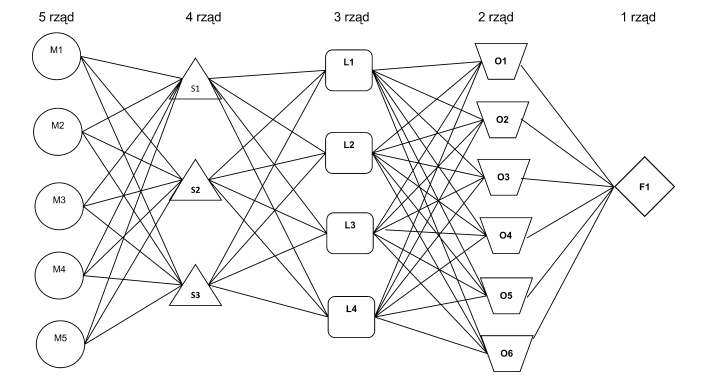
\includegraphics[width=\linewidth]{pictures/siec.png}
  \caption{Przykładowa sieć relacji w łańcuchu logistycznym}
  \label{fig:siecKawa}

\end{figure}

W niniejszej pracy stosowane jest rozszerzenie tego podejścia, poprzez zaprogramowanie jako agentów jednostek organizacyjnych przedsiębiorstwa \textit{(fabryka, magazyn, sklep, zarząd)}, które razem tworzą system \textit{(przedsiębiorstwo)}. 

To podejście opiera się na obserwacji, że relacje pomiędzy jednostkami w przedsiębiorstwie są analogiczne do relacji uczestników łańcucha dostaw. \cite{Porter1985} zauważył, że działalność przedsiębiorstwa to de facto sekwencja działań, która na każdym ogniwie zwiększa wartość dla odbiorcy. Zasady funkcjononawia opisywanego przez Portera \textit{łańcucha wartości} są identyczne co do opisywanego przez \cite{Moyaux2006} i \cite{Kawa2010} łańcucha dostaw a relacje pomiędzy nimi można przedstawić w sposób zaproponowany przez \cite{Kawa2010} --- sieci neuronowej widocznej na wykresie \ref{fig:siecKawa}. Podobieństwo to podkreśla fakt, że przedsiębiorstwa poprzez strategię \textit{integracji wertykalnej} swym zasięgiem mogą w rzadkich przypadkach objąć całość łańcucha dostaw.  

Ponieważ przedsiębiorstwa często dysponują wieloma duplikującymi swoje działania jednostkami \footnote{Dobrym przykładem są tutaj zakłady samochodowe, które mogą produkować dany model w różnych krajach. Zmiana fabryki powoduje przy tym radykalną zmianę łańcucha dostaw}, łańcuch ten jest nieliniowy i w jego przypadku mamy do czynienia z podobnymi wyzwaniami co w łańcuchu logistycznym.

Zdefiniowanie jako agentów poszczególnych jednostkek przedsiębiorstwa jest przy tym spójne z określoną przez \cite{Wooldridge1995} charakterystyką agenta, który według ich postulatów posiada : 
	\begin{itemize}
		\item autonomię --- poszczególne jednostki przedsiębiorstwa podążają za strategią i celami narzuconymi przez zarząd, ale mają zazwyczaj swobodę w podejmowaniu decyzji mających na celu ich realizację,
		\item zdolności do komunikacji --- jednostki przedsiębiorstwa komunikują się z otoczeniem (relacje z klientami) oraz między sobą (raportowanie do zarządu, spotkania), a w ramach pomiędzy jednostkami przedsiębiorstwa istnieje asymetria informacji,
		\item reaktywność --- jednostki przedsiębiorstwa reagują na zmiany rynkowe oraz zmiany wewnętrz przedsiębiorstwa,
	 	\item proaktywność --- jednostki przedsiębiorstwa podejmują inicjatywy mające na celu zwiększyć wartość przedsiębiorstwa, jak działalność innowacyjna bądź ekspansja. 
	\end{itemize}
 
 Dlatego w niniejszej pracy będziemy rozważać model wieloagentowy, w którym według założeń na przedsiebiorstwo składać się będzie szereg autonomicznych agentów,
	\begin{itemize} 
		\item $n$ \textit{fabryk} $\in$ $FA = \{fa_1,fa_2,fa_3..fa_m\} $ 
		\item $k$ \textit{magazynów} $\in$ $MA = \{ma_1,ma_2,ma_3..ma_k\} $ 
		\item $i$ \textit{sklepów} $\in$ $SK = \{sk_1,sk_2,sk_3..sk_i\} $
		\item oraz \textit{zarządu}, pełniący rolę centralnego koordynatora
	\end{itemize}

przez które kolejno będzie musiał przejść produkt zanim będzie mógł być zakupiony przez klienta. Rozpatrując ten system w proponowanym przez \cite{Kawa2010} kontekście teorii grafów oznacza to, że w przedsiębiorstwie istnieć będzie $m$ łańcuchów dostaw $d$, których ilość będzie równa  $n\choose 1 $ $ \times $ $k\choose 1 $ $ \times $ $i\choose 1 $ kombinacji połączeń pomiędzy jednostkami przedsiębiorstwa. Jak zauważa \cite{Kawa2010}, każde z tych połączeń będzie miało swoją maksymalną przepustowość oraz koszt $k_d = f(d)$, zależny od łańcucha i będący sumą kosztów ponoszonych na każdym z ogniw łańcucha wartości. Na krańcach grafu może dojść do sprzedaży towaru i przychodu dla całego systemu --- jednak zaopatrzenie sklepu w zbyt dużą ilość towaru doprowadzi do jego zmarnowania i strat. 

\subsubsection{Zadanie optymalizacyjne} 
Optymalizując działanie przedsiębiorstwa będziemy dążyć do tego, żeby dla danego poziomu produkcji $x$ i zbioru \textit{produktów} $PR = \{pr_1,pr_2,pr_3..pr_x\} $ ze zbioru możliwych sterowań (możliwych tras dostawy) $<d_1,d_2,d_3..d_m>$ dla każdego z produktów wybrać trasy maksymalizujące wyrażenie

\begin{equation} \label{eq:teoria1}
\max \sum\limits_{pr=1}^x  zysk (p,d) = p \times q - k_d \\
\end{equation}

\begin{center}
 gdzie $k_d = f(d)$, $p$ to cena, $d$ to wybrana droga \\
 a $q$ to sprzedaż zapisana jako zmienna binarna
\end{center}

Ponieważ kluczowym elementem powyższego równania jest zmienna $q$ i to, czy przyjmie wartość 1 czy 0 \footnote{Zmienna przyjmuje wartość 1 jeśli towar znalazł nabywcę i 0 jeśli nie został sprzedany, tak więc dla niesprzedanych towarów przedsiębiorstwo odnotuje koszty bez przychodów.} to zadanie optymalizacyjne byłoby względnie proste, gdybyśmy mieli doskonałą informację na temat poziomu sprzedaży w każdym ze sklepów w chwili $ t + 1 $. Na taką wiedzę nie możemy liczyć ani w tej pracy, ani w w rzeczywistości, dlatego rozwiązaniem proponowanym w niniejszej pracy jest zastosowanie modelowania predykcyjnego (\textit{predictive analytics}), w celu prognozowania liczby klientów i ich wyborów w każdym ze sklepów w najbliższych okresach czasu. \footnote{Obecnie w przedsiębiorstwach rzadko stosuje się zaawansowane sposoby prognozowania sprzedaży (\textit{predictive analytics}), a zarządzanie dostawami odbywa się raczej metodą manualnego uzupełniania zapasów.} 

Ponadto, jak warto zauważyć, nie możemy liczyć na to, że funkcja kosztu $k_d$ będzie liniowa. Wspominana przez \cite{Kawa2010} maksymalna przepustowość każdego z łańcuchów, która w przedsiębiorstwie będzie spowodowana ograniczonymi mocami produkcyjnymi, może spowodować, że funkcja kosztu będzie funkcją wypukłą \footnote{Wyprodukowanie każdego kolejnego produktu ponad moc produkcyjną będzie wymagało nadgodzin, dodatkowej przestrzeni magazynowej, pomocy poddostawców - a każde z tych wydarzeń będzie generowało dodatkowe koszty.}. W niektórych przypadkach mogą istnieć także korzyści skali, które spowodują, że funkcja będzie funkcją wklęsłą, a całkiem realne jest istnienie obu tych efektów  \footnote{Korzyści skali odczuwalne do pewnego optymalnego poziomu produkcji, powyżej którego brak mocy produkcyjnych powoduje  powiększanie się kosztów krańcowych.}, przez co musimy zakładać, że $f(d)$ może być dowolną funkcją nieliniową.

Trzecim aspektem który trzeba wziąć pod uwagę jest złożoność obliczeniowa. Nawet dla prostego układu, lecz wolumenu produkcji ponad 1000 sztuk sprawdzenie zysku w przypadku wszystkich kombinacji alokacji wymaga olbrzymiej ilości iteracji. Mimo znaczącego wzrostu mocy komputerów w ostatnich latach, wolumeny produkcji w dużych przedsiębiorstwach oraz złożoność tras logistycznych sprawia, że to podejście jest kompletnie niepraktyczne i należy szukać alternatywnych podejść, upraszczających problem.

 Proponowany algorytm będzie brał wszystkie te aspekty pod uwagę, a pierwszy z wymienionych problemów rozwiążemy wykorzystując  \textit{modelowanie predykcyjne}.

\subsubsection{Modelowanie predykcyjne} \label{statistical} 
Jak wskazuje \cite{James2013}, zakładając, że dysponujemy zbiorem $n$ obserwacji $p$ zmiennych, możemy zbadać ich relację ze zmienną wyjaśnianą $y$ i otrzymać \textit{model}, który dla nowych - nieanalizowanych wcześniej - obserwacji $x_1,x_2..x_n$  zwraca przewidywaną wartość zmiennej objaśnianej \^{y}. Różnorodne metody dzięki którym możemy otrzymać zmienną objaśnianą \^{y} \cite{James2013} nazywa \textit{statistical learning}, i zaznacza, że mogą one być wykorzystane do modelowania predykcyjnego, tj. przewidywania przyszłych wydarzeń na podstawie przeszłej historii danych. 

Zastosowanie metod \textit{statistical learning} w przedsiębiorstwach potwierdza \cite{Buckinx2007}, który wskazywał na możliwość prognozowania lojalności klienta na podstawie wewnętrznych danych o transakcjach, oraz \cite{Davenport2011}, który opisuje szereg  \textit{case studies} firm, w których wykorzystuje się istniejące dane o transakcjach do przewidywania przyszłych zakupów klientów. Jednym z podanych przez niego przykładów jest Tesco, które na podstawie zebranych danych przewiduje, jak będzie wyglądał koszyk zakupów klienta podczas następnych zakupów, i odpowiednio wcześnie wysyła mu bony zniżkowe. Również podczas panelu \textit{Strategia B2C w erze Big Data - jak wykorzystać potencjał danych} na XXV Forum Ekonomicznego w Krynicy przedstawicielie polskiego biznesu zwracali uwagę na szerokie wykorzystanie modelowania predykcyjnego również w nasz gospodarce. \footnote{Jednak jak zwracano uwagę, \textit{big data}\ i \textit{modelowanie predykcyjne}\ służą głównie do zyskiwania wiedzy o kliencie i rynku do manualnego przetworzenia \textit{insight}\ , a nie automatyzacji podejmowania decyzji, co rozważamy w tej pracy}

Podane przykłady dają nam podstawy, żeby w przypadku optymalizowanego przedsiębiorstwa zakładać, że dane o każdej transakcji są zapisywane wraz z niektórymi danymi osobowymi klienta \footnote{To stwierdzenie opiera się na opisywanym przez \cite{Davenport2011} przypadku Tesco i zastosowanej przez nich metody zbierania danych. Możliwość zbierania danych o transakcjach określonego klienta daje karta lojalnościowa (lub konto, w przypadku e-commerce), na którą rejestrowana jest każda transakcja. Praktyką jest, żeby przy okazji tworzenia karty lojalnościowej zbierać informacje o kliencie w ankiecie (zakres danych zależy od praktyki korporacyjnej). Dzięki temu, przedsiębiorstwa są w stanie przypisać do zakupów dane osobwe jak płeć, miejsce zamieszkania, wykształcenie etc.}, a cały zbiór danych może być wykorzystany do przewidywania sprzedaży w chwili $t + 1$. 

Dla każdej transakcji w sklepie dysponujemy więc zbiorem informacji $ X = n \times x_i = <tr_1..tr_k, pr_1.. pr_k,kl_1..kl_k>$ gdzie $tr$ to identyfikatory transakcji (miejsce, data, rodzaj płatności), $pr$ to identyfikatory produktu (nazwa, cena, ilość) oraz $kl$ to identyfikatory klienta (płeć, wiek, zarobki, wykształcenie etc.). 

Na podstawie takiego zbioru danych chcemy przewidzieć popyt na produkty w każdym ze sklepów, co w praktyce oznacza konieczność stworzenia modelu estymującego następujące wielkości

	\begin{itemize} 
		\item liczność $n$ poszczególnych grup klientów \footnote{Przez \textit{poszczególne grupy klientów} rozumiemy klientów o wspólnej charakterystyce, czyli takich samych zestawach zmiennych identyfikujących $<kl_1..kl_n>$} odwiedzających sklep w chwili $t+1$, gdzie \^n $\in R$ 
	\end{itemize}
	oraz, w zależności od zastosowanego podejścia,
	\begin{itemize} 
		\item prawdopodobieństwo $p$ z jakim klient o danej charakterystyce kupi produkt $pr$, gdzie \^{p} $\in (0,1)$  
		\item produkt wybrany przez danego klienta, gdzie \^{pr} $\in \{pr_1,pr_2..pr_n\}$, a $pr_i$ to dostępny produkt.
	\end{itemize}

Jak wskazuje \cite{James2013}, zmienna objaśniana może przyjąć różne dziedziny --- m.in. zmiennej binarnej (1/0), prawdopodobieństwa, \textit{log odds} lub klasy --- i z tego względu każdy z przypadków różni się metodami które możemy zastosować. Według sugestii \cite{James2013} i \cite{hastie2001} , zastosujemy następujące metody

	\begin{itemize} 
		\item do liczby klientów - regresję metodą OLS (\textit{ordinary least squares, metoda najmniejszych kwadratów})
		\item do prawdopodobieństwa zakupu - regresję logistyczną (\textit{logistic regression})
		\item do wyboru produktu- metody klasyfikacyjne \textit{k-means} oraz \textit{drzewa klasyfikacyjne}
	\end{itemize}
	oraz metody nie służące bezpośrednio do modelowania \^{y}, jednak wspierające proces predykcyjny
	\begin{itemize} 
		\item pomiar odległości \textit{distance scaling}, poprzez liczenie odległości euklidesowej (\textit{euclidean distance}) pomiędzy dwoma zbiorami danych i stworzenie obliczenie macierzy niepodobieństwa (odległości, \textit{dissmiliarity matrix}
		\item eliminację zmiennych (\textit{backward elimination}, która jest jednym z podejść wyboru podzbiorów (\textit{subset selection}) do selekcji zmiennych wyjaśniających które wspólnie tworzą najlepszy model
		\item prawdopodobieństwo warunkowe do przewidywania, jacy konsumenci odwiedzą sklep w $t+1$, a co za tym idzie, jakie są wartości zmiennych objaśniających do prognozowania  \^{y}
	\end{itemize}	


\newpage

\subsection{Proponowany algorytm optymalizacyjny} 
Znając przewidywaną sprzedaż na krańcach grafu, proponowany w niniejszej pracy algorytm rozwiązania powyższego problemu opiera się na obserwacji, że równanie \ref{eq:teoria1} będzie równoważne zapisowi sumującemu po możliwych kombinacjach łańcucha, zamiast dla każdego produktu z osobna. Nie tylko znacząco zmniejszy to liczbę potrzebnych iteracji obliczeń \footnote{Ze względu na bardzo duży wolumen produkcji w opisywanej branży FMCG, mało prawdopodobne jest, aby liczba kombinacji tras dostaw była większa od liczby produktów, ale nawet wówczas istnieje możliwość rozważania tylko predefiniowanego zestawu tras), ale także umożliwi dalsze obliczenia upraszczające problem.}

\begin{equation}  \label{eq:teoria2}
\max \sum\limits_{d=1}^m  zysk(p) = 
p \times pr_d -  \ k_d \times pr_d \qquad 
\end{equation}

\begin{center}
  gdzie $pr_d$ to ilość produktów przechodzącym przez dany łańcuch, \\ 
  a $k_d$ to funkcja kosztu $f(d)$
\end{center}

Ponieważ scieżka $d$ składa się z kombinacji jednostek przedsiębiorstwa wchodzących w jej skład, czyli $<fa,ma,sk>$, koszt ponoszony na całej trasie będzie równie sumie kosztów ponoszonym na każdym z ogniw łańcucha, a równanie \ref{eq:teoria2} możemy zapisać jako

\begin{equation} \label{eq:teoria3}
\max \sum\limits_{d=1}^m  zysk(p) = 
p \times pr_d -  ( \sum\limits_{j=1} k_j) \times pr_d \qquad 
\end{equation}

gdzie $ k_j$ to funkcja kosztu każdego z elementów łańcucha wartości (koszty produkcji, magazynowania, transportu, etc.). Warto odnotować przy tym, że zgodnie z założeniami funkcja $k_j$ ze względu na efekty skali może być nieliniowa. Zakładamy, że funkcja ta jest nam znana, więc zostaje nam znalezienie takich wartości $pr_d$ i \textit{ceny} (jeśli nie przyjmujemy założenia danej, stałej ceny) dla których firma będzie osiągać maksymalny zysk. Ze względu na występujące w przedsiębiorstwie współzależności oraz nieliniowość kosztów (korzyści skali) musimy cały układ rozważać łącznie. 

Na przykładzie przedsiębiorstwa będącego zbiorem jednostek $<fa_1, ma_1, ma_2, sk_1, sk_2, sk_3>$ mamy do czynienia z $m= $ $1\choose 1 $ $ \times $ $2\choose 1 $ $ \times $ $3\choose 1 $ = 6 kombinacji połączeń pomiędzy jednostkami przedsiębiorstwa, przy czym każdy do każdego ze sklepów można przeprowadzić dostawę jedną z dwóch tras. \\ 

\begin{center}
\begin{tikzpicture}
   % Draw all levels

  \draw[level] (0,0) -- node[above] {fabryka  $fa_1$} node[below] {($k_{fa_1}$)}  (2,0);

  \draw[connect] (2,0)  -- (3,-1) (2,0) -- (3,1);
  \draw[level]   (3,1)  -- node[above] {magazyn  $ma_1$} node[below] {($k_{ma_1}$)} (5,1);
  \draw[level]   (3,-1) -- node[above] {magazyn $ma_2$} node[below] {($k_{ma_2}$)} (5,-1);

  \draw[connect] (5,1)    -- (6,2) (5,1) -- (6,0) (5,1) -- (6,-2) (5,1) ;
  \draw[connect] (5,-1)    -- (6,2) (5,-1) -- (6,0) (5,-1) -- (6,-2) (5,-1);

  \draw[level]   (6,2)  -- node[above] {sklep $sk_1$} node[below] {($k_{sk_1}$)}  (8,2); 
  \draw[level]   (6,-2)  -- node[above] {sklep $sk_2$}node[below] {($k_{sk_1}$)}  (8,-2);
  \draw[level]   (6,0)  -- node[above] {sklep $sk_3$}node[below] {($k_{sk_1}$)}  (8,0);

  \draw[connect_k] (8,2)    -- (8.5,2.5) (8,2) -- (8.5,1.5) (8,2);
  \draw[connect_k] (8,0)    -- (8.5,0.5) (8,0) -- (8.5,-0.5) (8,0);
  \draw[connect_k] (8,-2)    -- (8.5,-2.5) (8,-2) -- (8.5,-1.5) (8,-2);

  \node[text width=4cm] at (10.75,2.5) {  $ _{1.} k_{d_1}  $};
  \node[text width=4cm] at (10.75,1.5) {  $ _{2.} k_{d_2}   $};
  \node[text width=4cm] at (10.75,0.5) {  $ _{3.} k_{d_3}   $};
  \node[text width=4cm] at (10.75,-0.5) {  $ _{4.} k_{d_4} $};
  \node[text width=4cm] at (10.75,-1.5) {  $ _{5.} k_{d_5}  $};
  \node[text width=4cm] at (10.75,-2.5) {  $ _{6.} k_{d_6} $};

  % Draw labels
  \node[label] at (1,3.5)  {\textit{Fabryki}};
  \node[label] at (4,3.5)  {\textit{Magazyny}};
  \node[label] at (7.5,3.5)  {\textit{Sklepy}};
  \node[label] at (10.75,3.5)  {\textit{Trasy}};

  % Draw annotations
\end{tikzpicture}
\end{center}

Ponieważ przewidywany wolumen sprzedaży produktu w każdym z krańców grafu jest nam znany \footnote{Zakładamy, że dzięki \textit{Predictive analytics} na podstawie poprzednich obserwacji mamy dokładne prognozy dotyczące sprzedaży w chwili $t+1$}, żeby umożliwić obliczenie optymalnego obłożenia każdej z tras prowadzącej do krańcu grafu \footnote{Żeby ograniczyć złożoność obliczeniową staramy się unikać pętli, która sprawdza każdą kombinację, zamiast tego szukając bardziej wyrafinowanych sposobów} możemy dla każdej z tras ilość przechodzących nią produktów zapisać jako 

\begin{equation*}
pr_1 = \alpha pr_{sk_1} , \quad pr_2 = \beta pr_{sk_1} \quad ... \quad  pr_{d-1} = \gamma pr_{sk_i} ,\quad  pr_d = \delta  pr_{sk_i}
\end{equation*}

gdzie $pr_{sk_d}$ to ilość produktów, jakie mają trafić do $sk_d$ krańca grafu leżącego na trasie $d$, a $\alpha,\beta...\delta$ to udział tej trasy w przepływie wszystkich towarów do danego krańca grafu. W ten sposób, równanie  \ref{eq:teoria3} możemy zapisać jako 

\begin{equation} \label{eq:teoria4}
\max \sum\limits_{d=1}^m  zysk(cena) = 
cena \times \alpha pr_{sk_d}-  ( \sum\limits_{j=1} k_j) \times \alpha pr_{sk_d} \qquad 
\end{equation}

Co po rozwinięciu pozwoli nam na sprowadzeniu równania \ref{eq:teoria4} do postaci

\begin{multline} \label{eq:teoria5}
zysk(cena) = \alpha(cena \times pr_{sk_1} - ( \sum\limits_{j=1} k_j) \times pr_{sk_1}) + \\
 ... \ + \delta(cena \times pr_{sk_i} - ( \sum\limits_{j=1} k_j) \times pr_{sk_1})
\end{multline}


jeśli przyjmiemy, że  

\begin{multline*}
a = (cena \times pr_{sk_1} - ( \sum\limits_{j=1} k_j) \times pr_{sk_1}) ... \\
.. b=(cena \times pr_{sk_i} - ( \sum\limits_{j=1} k_j) \times pr_{sk_1})
\end{multline*}

otrzymamy w ten sposób wieloman, w którym współczynniki $a,b$ są nam znane \footnote{$pr_{sk_1}$ zostały wyprognozowane modelowaniem predykcyjnym, a $k_j$ to znana nam suma funkcji kosztów w każdej jednostce}, a pary współczynników $\alpha, \beta$ jednego krańca grafu muszą być mniejsze lub równe 1. \footnote{Warunkiem nie jest "równe 1", ponieważ może istnieć taki udział $\alpha$ w przedziale $<0,1>$ powyżej którego przez nieliniowość funkcji kosztów dostawa może być nieopłacalna}. 

Za Sydsaeter, 2005 zauważmy, że $\frac{\partial zysk}{\partial \alpha} , \frac{\partial zysk}{\partial \beta} ... \frac{\partial zysk}{\partial \delta}$ - czyli pierwsze pochodne cząstkowe po $\alpha,\beta,\delta$ z tak zdefiniowanej funkcji - dadzą nam informację, o ile wzrośnie zysk przedsiębiorstwa w przypadku zwiększenie obłożenia tej trasy. Dlatego dla każdego produktu $pr_n$ istnieje możliwość wybrania takiej z tras $<d_1,d_2,d_3..d_m>$, która będzie maksymalizowała wynik przedsiębiorstwa - jak w równaniu \ref{eq:teoria1}. 

Algorytm będzie więc działał jak zostało to pokazane na wykresie \ref{fig:diagramoptymalizacyny}

\begin{figure}
  \centering
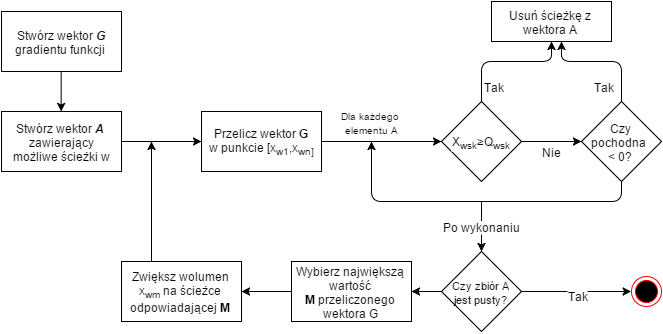
\includegraphics[width=\linewidth]{pictures/diagramoptymalizacyny.png}
  \caption{Proponowany algorytm optymalizacyjny}
  \label{fig:diagramoptymalizacyny}

\end{figure}

% --- chapter ---------------------------------------------------------
\clearpage

\section{Model}

W celu sprawdzenia działania algorytmu zbudowany został model wieloagentowy, który symuluje lokalny rynek na wybrany produkt, wraz z zachowaniami konsumentów i funkcjonowaniem przedsiębiorstwa.

\subsection{Koncepcja modelu}

Zgodnie z argumentacją zawartą w rozdziale \ref{teoria}, relacje w przedsiębiorstwie pomiędzy jednostkami tworzącymi wspólnie łańcuch dostaw można przedstawić jako model wieloagentowy. Jednocześnie, inspirując się \cite{Kaminski2012}, zakładamy, że możemy stworzyć zbiór heteregenicznych agentów symulujących decyzje konsumentów w celu modelowania rynku. Łącząc te podejścia, celem pracy jest stworzenie modelu wieloagentowe symulującego rynek (w szczególności aspekt sprzedaży oraz dostaw) na którym moglibyśmy sprawdzić wpływ działania algorytmu na wyniki przedsiębiorstwa.

Zgodnie z powyższym, w modelu znajdą się następujący typy agentów: 

\begin{itemize} 
	\item \textbf{klienci}, który zgodnie z założeniem będą heterogeniczni i definiowani przez cechy demograficzne \footnote{Są to między innymi wiek, zarobki, wykształcenie, zainteresowania - zostanie to dokładnie opisane w dalszej części pracy.}, które wpływającą na podejmowane przez niego decyzje oraz zachowania, 
	\item \textbf{przedsiębiorstwo}, sprzedające \textit{produkt} na rynku. Zgodnie z podejściem przedstawionym w \ref{teoria}, przedsiębiorstwo będzie rozumiane jako zbiór niezależnych, współpracujących ze sobą agentów 
		\begin{itemize}
			\item fabryk
			\item magazynów
			\item sklepów 
			\item zarządu, pełniącego funkcje koordynującą 
		\end{itemize}
	\item \textbf{konkurencji}, zachowującej się pasywnie w stosunku do rynku, konsumentów i symulowanego przedsiębiorstwa, ale wprowadzajacej na rynek szereg produktów stanowiących alternatywę dla produktu symulowanej firmy \footnote{Tj. konkurencja nie zmienia decyzji podjętych przed rozpoczęciem gry, i w założeniu ma stanowić jedynie alternatywę dla konsumentów.} 
	\item \textbf{produktów} dostępnych na rynku, z których każdy zdefiniowany jest unikalnymi cechami określającymi jakość, typ i cenę produktu, przez co każdy z produktów będzie preferowany przez inną grupę konsumentów, a preferencje są oparte na danych ze świata rzeczywistego. 
\end{itemize}

\paragraph{Aspekt lokalizacji}\mbox{}\\

Aby dobrze odwzorować kluczowy aspekt lokalizacji i dróg w łańcuchach dostaw, symulowany rynek jest osadzony w \textit{wirtualnym mieście}. Oznacza to, że każdy agent ma swoją lokalizację w macierzy o wymiarach $x \times y$ i może się w niej poruszać po wyznaczonych drogach.

Lokalizacja wpływa na działania agenta - klient kupi produkt tylko w sklepie który będzie na jego ścieżce, a dostawa z magazynu do sklepu będzie tym droższa, im bardziej oddalone będą od siebie. 

\paragraph{Symulowanie decyzji konsumenckich}\mbox{}\\

W modelu konsumenci nieustannie poruszają się po \textit{mapie}, bez związku z działaniem przedsiębiorstwa \footnote{W każdej jednostce czasu $t$ chodzą do pracy i odwiedzają znajomych}. W każdej jednostce czasu $ t $ klienci z prawdopodobieństwem $ p $ będą potrzebować symulowany produkt, więc odwiedzą któryś ze sklepów będących na ich trasie w czasie $t$, i wybiorą jeden z produktów oferowanych przez przedsiębiorstwo i konkurencję. 

Symulacja wyboru opiera się na danych o preferencjach konsumenckich zebranych w ankiecie na próbie 169 badanych, w wyniku których otrzymano 1860 rekordów danych. Na ich podstawie których zbudowane zostało drzewo klasyfikacyjne opisujące prawdopodobieństwo zakupu produktu od cech konsumenta. 

Ponieważ każdy konsument-agent w modelu ma swoje unikalne cechy demograficzne i charakteru, wykorzystujemy zbudowane drzewo klasyfikacyjnego do określenia wyboru, jakiego najprawdopodobniej dokonał by jego odpowiednik w świecie rzeczywistym. \footnote{Oczywiście, o wiele lepsze byłoby oparcie pracy o prawdziwe historie transakcji, jednak jest to niemożliwe ze względu na dużą poufność tych danych} Przeprowadzając podobny proces dla każdego konsumenta w modelu, otrzymujemy dynamiczną symulację rynku produktów szybkozbywalnych. 

\paragraph{Decyzje przedsiębiorstwa}\mbox{}\\

Ponieważ konsument wybiera produkt tylko z gamy dostępnych w sklepie, kluczowe dla sukcesu przedsiębiorstwa jest dostarczenie w każdej jednostce czasu $t$ odpowiedniej ilości produktów \footnote{W warunkach symulacji nie można zapełnić \textit{półek sklepowych} do pełna, bo brak sprzedaży oznacza stratę dla przedsiębiorstwa, a w sektorze FMCG zakładamy, że w czasie $t+1$ produkty stracą zdolność do spożycia}. Oznacza to, że przed rozpoczęciem każdej tury przedsiębiorstwo musi podjąć szereg decyzji o m.in.
	\begin{itemize}
		\item odpowiednim poziomie produkcji,
		\item wolumenie dostaw do każdego ze sklepów w sieci,
		\item rozdzieleniu wolumenów pomiędzy części przedsiębiorstwa, tj. ile z całkowitego wolumenu ma wyprodukować fabryka $A$, a ile fabryka $B$
	 	\item jaką trasą powinny zostać wysłane dostawy do każdego ze sklepów. \footnote{Rozumiemy przez to pytanie, który z magazynów ma być pośrednikiem, ponieważ dobra nie mogą być dostarczane bezpośrednio z fabryki do sklepu.}
	\end{itemize}

Każda z tych decyzji będzie miała wpływ na przychody \footnote{Przy założeniu stałej ceny, będą to przede wszystkim \textit{utracone koszty} w przypadku wyczerpania się zapasów w sklepie} oraz koszty firmy. Celem pracy jest zbudowanie algorytmu, który na podstawie dotychczasowej historii transakcji pozwoli symulowanemu przedsiębiorstwu przewidzieć potencjalną sprzedać w czasie $ t +1 $ i ze zbioru możliwych sterowań (wyżej wymienionych decyzji) $<u_{t+1}>$ wybierze takie, które będą maksymalizować zysk. 

\subsection{Zastosowane narzędzia}

Model został zbudowany w języku programowania Python 2.7, z wykorzystaniem następujących bibliotek: 

\begin{center}
\begin{tabular}{lccc}
 Biblioteka & Źródło & Zastosowanie \\ 
\hline
 Sympy & www.sympy.org & Wykorzystanie do obliczeń symbolicznych \\  
 scikit-learn & scikit-learn.org & Wykorzystanie bibliotek metod statystycznych \\ \hline
\end{tabular}
\end{center}

Kod programu dostępny jest pod adresem  \textit{github.com/hubertguzera/master-thesis}

\subsection{Struktura programu}

Program podzielony jest na trzy moduły, jak zaprezentowano na rysunku \ref{fig:struktura}

	\begin{itemize}
		\item Pierwsza odpowiada za stworzenie, w drodze losowań, środowiska w ramach którego toczy się symulacja, wraz z agentami i macierzą lokalizacji. \footnote{Model może pominąć tą część i wczytać pregenerowany świat w celu sprawdzenia różnych scenariuszy w statycznym świecie (ceteris paribus).}
		\item  Druga część przez $t_n$ jednostek czasu symuluje działanie rynku --- decyzji klientów i funkcjonowania przedsiębiorstwa --- według predefiniowanych zasad sterowań \footnote{Co istotne, algorytm optymalizacyjny jeszcze nie jest implementowany na tym etapie}, zwracając na koniec wyniki (przychody, koszty i zysk) przedsiębiorstwa w danej jednostce czasu $t$.
		\item Trzecia po $t_n$ rund symulacji aplikuje algorytm optymalizacyjny, który poprzez prognozowanie sprzedaży na krańcach grafu w $t_{n+1}$, szuka najlepszych decyzji o alokacji produktów. Działanie algorytmu można porównać do miary porównawczej uzyskanej w pkt 2. 
	\end{itemize}

\begin{figure}
  \centering
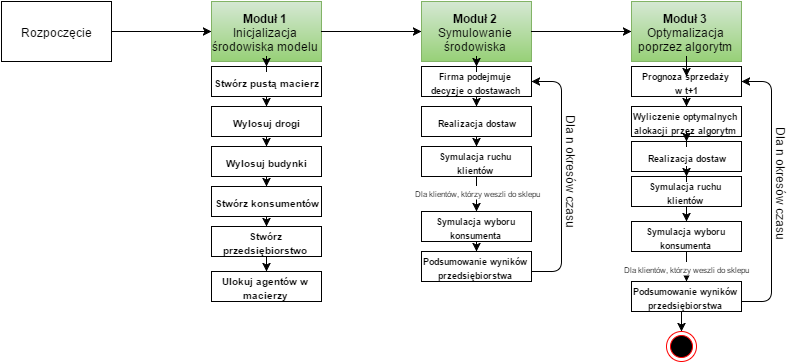
\includegraphics[width=\linewidth]{pictures/Struktura.png}
  \caption{Struktura działania programu}
  \label{fig:struktura}
\end{figure}


\subsection{Generowanie środowiska modelu}
\paragraph{Klasa \textit{rynek}}\mbox{}\\
Za reprezentację tak opisanego środowiska modelu odpowiada klasa \textit{rynek}, wobec której dziedziczą wszystkie inne klasy występujące w modelu. Klasa \textit{rynek} i wszystkie dziedziczone jest generowana dynamicznie i losowo, jednak może być zapisana jeśli istnieje konieczność replikacji obliczeń albo porównań.  Konstrukcja klasy \textit{rynek} w programie została zaprezentowana w diagramie \ref{rynek}. \\

\begin{tikzpicture} \label{rynek}
\begin{class}[text width=11cm]{rynek}{0,0}
\attribute{swiat : class}
\attribute{symulowana\_firma : class}
\attribute{tura : integer}
\attribute{produkty\_na\_rynku : class}

\operation{\_\_init\_\_(self,swiat) : None}
\operation{sprzedaz\_w\_sklepach(self) : None}
\operation{nowatura (self) : None}
\end{class}
\end{tikzpicture}

\paragraph{Klasa \textit{świat}}\mbox{}\\

Klasa \textit{swiat} zawarta w klasie \textit{rynek} powstała w celu odpowiedniego odwzorowania kluczowego aspektu lokalizacji i dróg w łańcuchach dostaw, wzorując się na podejściu zastosowanym w \textit{modelu segregacji Schellinga} (\cite{Schelling1971}). Agenci osadzoni są w przestrzeni, reprezentowaną przez macierz klas \textit{lokalizacja} o wymiarach (x,y). Dodatkowo, lokalizacje są połączone drogami, wymusząjąc na agentach poruszanie się tylko w obrębie ścieżek. Dzięki temu, w modelu będziemy mogli wiernie odwzorować wpływ odległości i wyboru trasy na efektywność procesów logistycznych, oraz zależność wyników sklepu od zamieszkującej okolicę populacji. 

Macierz \textit{mapa} generowana jest generowana jest według algorytmu widocznego na rysunku \ref{fig:lokalizacje}, który gwarantuje następujące właściwości otrzymanej w ten sposób macierzy lokalizacji. 

	\begin{itemize}
		\item Drogi krzyżują się i skręcają tylko pod kątem prostym. Poza skrzyżowaniami, drogi nie mają w sąsiedztwie innych dróg,
		\item Inne lokalizacje (domy, sklepy etc.) mogą występować tylko w bezpośrednim sąsiedztwie drogi,
		\item Drogi stanowią ciągłą linię, dzięki czemu nie ma punktu, do którego nie dałoby się dojechać z dowolnego miejsca startowego,
		\item W regione 2 punktów od skraju mapy nie są generowane ani drogi, ani lokalizacje.  \footnote{Jest to zabezpieczenie algorytmu, który w odległości 2 pkt od skraju mapy ma 0 proc. szansy na poprowadzenie ścieżki dalej - ponieważ w przypadku iterowania na skrajach mapy niektóre funkcje (jak sprawdzenie sąsiadujących punktów) mogą odnieść się do lokalizacji poza macierzą, powodując błąd programu}
	 	\item Gęstość sieci dróg oraz prawdopodobieństwo występowania zakrętów jest predefiniowana przez użytkownika
	\end{itemize}

Przykładowa \textit{mapa} otrzymana w wyniku działania algorytmu widoczna jest na rysunku \ref{fig:mapa}.
 \\

\begin{tikzpicture}
\begin{class}[text width=11cm]{swiat}{-1,0}
\attribute{mapa : array \textit{--- macierz lokalizacji o wymiarach x,y}}
\attribute{ludnosc : array type \textit{--- macierz instacj klasy konsument}}
\attribute{ludnosc : dictionary \textit{--- slownik sieci drog}}
\end{class}

\begin{class}[text width=7cm]{lokalizacja}{-5,-5}
\inherit{swiat}
\attribute{typ : string \textit{--- typ budynkui}}
\attribute{x : integer \textit{--- lokalizacja x}}
\attribute{y : integer  \textit{--- lokalizacja y}}
\attribute{droga : array \textit{--- przylegla droga}}
\end{class}

\begin{class}[text width=7cm]{konsument}{3,-5}
\inherit{swiat}
\attribute{plec : string}
\attribute{wiek : integer}
\attribute{zarobki : integer}
\attribute{zainteresowania : array}
\attribute{wyksztalcenie : integer}
\attribute{okazja : boolean}
\attribute{domx : integer}
\attribute{domy : integer}
\attribute{pracax : integer}
\attribute{pracay : integer}
\operation{odwiedzony\_sklep(self,swiat) : None}
\operation{macierz\_cech(self) : array}
\end{class}
\end{tikzpicture}

\begin{figure}
  \centering
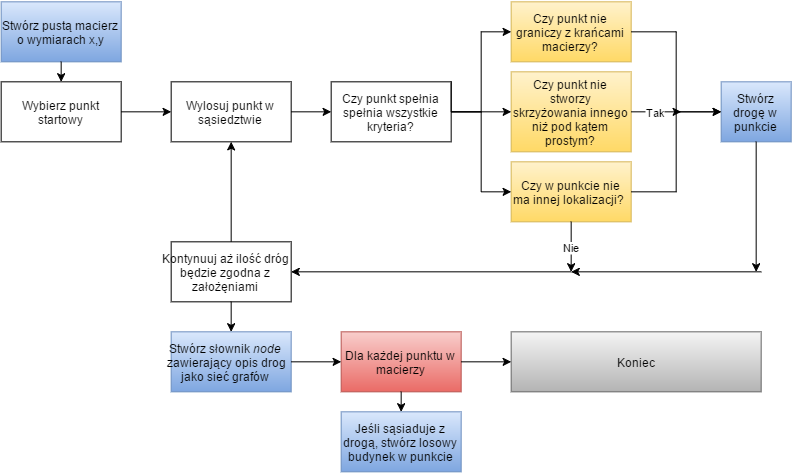
\includegraphics[width=\linewidth]{pictures/tworzeniedrog.png}
  \caption{Algorytm tworzenia dróg i lokalizacji}
  \label{fig:lokalizacje}
\end{figure}

\begin{figure} 
  \centering

\includegraphics[width=\linewidth]{../mapy/po_lokalizacji_sklepow.png}
  \caption{Przykładowa mapa - \textit{szary} to drogi, \textit{niebieski} - domy mieszkalne, \textit{czerwony} i \textit{zielony} - biurowce, \textit{pomarańczowy} - sklepy, \textit{żółty} - magazyny, \textit{błękitny} - fabryki}
  \label{fig:mapa}
\end{figure}


\subsubsection{Algorytm wyszukiwania drogi} 

Trasy pomiędzy zadanymi punktami w modelu są wyszukiwane dynamicznie, na podstawie algorytmu wyszukiwania drogi. Odległości z kolei obliczane są poprzez sumowanie ilości punktów w zwracanym przez algorytm łańcuchu. 

Algorytm oparty jest na metodach wyszukiwania ścieżek w grafach, dzięki założeniu, że każda droga o współrzędnej (x,y) na mapie jest punktem grafu, który może sąsiadować z punktami o współrzędnych (x-1,y),(x+1,y),(x,y+1),(x,y-1) \footnote{Punkty (x-1,y-1),(x+1,y-1),(x+1,y+1),(x-1,y+1) wykluczamy przez wcześniejsze założenie, że drogi krzyżują się tylko pod katem prostym}, o ile również są drogrami. \footnote{Informacje o punktach i sąsiadujących przechowywane są w zmiennej nodes, która jesst słownikiem, dla każdego klucza - punktu na mapie - przechowuje informacje o sąsiadujących punktach, np. (3,2) = [(3,3)(4,3)].} \footnote{Pewnym ograniczeniem jest, że jako punkty grafu definiujemy tylko drogi, tak więc szukając trasy z punktu A do punktu B de facto szukamy trasy z drogi przy punkcie A do drogi przy punkcie B.}

Algorytm, udostępniony przez Python Foundation \footnote{https://www.python.org/doc/essays/graphs/} i zaprezentowany w tabeli \ref{szukaniedrogi} ma następujące cechy
	\begin{itemize}
		\item jest rekurencyjny,
		\item nie jest losowy,
		\item nie gwarantuje znalezienia najkrótszej trasy.
	\end{itemize}

\begin{lstlisting}[frame=single, label=szukaniedrogi]  
    def find_path(graph, start, end, path=[]):
        path = path + [start]
        if start == end:
            return path
        if not graph.has_key(start):
            return None
        for node in graph[start]:
            if node not in path:
                newpath = find_path(graph, node, end, path)
                if newpath: return newpath
        return None
\end{lstlisting}

\subsection{Agenci, ich rodzaje i właściwości}
\subsubsection{Konsumenci} 

Idąc za \cite{Kaminski2012}, w modelu stosujemy modelowanie rynku za pomocą heterogeniczne konsumentów. Stąd, każdy z konsumentów ma swoją unikalną charakterystykę rozumianą przez cechy demograficzne oraz cechy charakteru, które będą wpływać na jego wybory. 

W dodatku, chociaż agenci nieustannie poruszają się w ramach modelu, to pula lokalizacji w ramach których będą się przemieszczać jest zamknięta --- każdy z konsumentów będzie się przemieszczał tylko w wyniku zdarzenia, którym może być podróż do pracy albo odwiedziny znajomych. Ponieważ dla każdego z agentów miejsce pracy jest z góry określona, a pula znajomych zamknięta do trzech, każdy z agentów będzie przemieszczał się pomiędzy maksymalnie czterami lokalizacjami, tworząc pewne wzorce zachowań. 

Dzięki temu, odwzierciedlamy zjawisko ze świata rzeczywistego, że konsumenci zazwyczaj robią zakupy w ograniczonej liczbie sklepów będących po drodze bądz niedaleko. Jest to bardzo istotny warunek funkcjonowania modelu, ponieważ losowy dobór klientów uniemożliwiłby modelowanie predykcyjne.

Każdy będzie definiowany w klasie o następujących właściwościach \\

\begin{tikzpicture}
\begin{class}[text width=11cm]{konsument}{0,0}
\attribute{plec : string}
\attribute{wiek : integer}
\attribute{zarobki : integer}
\attribute{zainteresowania : array}
\attribute{wyksztalcenie : integer}
\attribute{okazja : boolean \textit{--- wskazanie powodu wyjścia z domu}}
\attribute{domx : integer \textit{--- współrzędna x domu}}
\attribute{domy : integer \textit{--- współrzędna y domu}}
\attribute{pracax : integer \textit{--- współrzędna x pracy}}
\attribute{pracay : integer \textit{--- współrzędna y pracy}}
\operation{odwiedzony\_sklep(self,swiat) : None}
\operation{macierz\_cech(self) : array}
\end{class}
\end{tikzpicture}

\begin{lstlisting}[frame=single]  
class konsument:   
	plec = string
	wiek = integer 
	zarobki = integer 
	zainteresowania = array # macierz trzech string 
	znajomi = array # trzy relacje z innymi agentami
	wyksztalcenie = integer # 5-stopniowa skala 
	okazja = boolean # wskazanie czy wychodzi z domu
	domx = integer # wspolrzedna x domu na mapie
	domy = integer # wspolrzedna y domu  na mapie
	pracax = integer # wspolrzedna x pracy na mapie
	pracay = integer # wspolrzedna y pracy na mapie
\end{lstlisting}

Wartości dla każdego z konsumentów są losowane niezależnie na podstawie rozkładów publikowanych przez Główny Urząd Statystyczny \cite{GUS2011} oraz danych firmy Sedlak\&Sedlak (\cite{Sedlak2013}) \footnote{Raporty firmy Sedlak\&Seldlak służyły do zbudowania tabeli prawdopodobieństwa wystąpienia danego wynagrodzenia w zależności od płci i wykształcenia. Reszta danych oparta na GUS} w celu zagwarantowania odzwierciedlenia struktury społeczeństwa. Ze względu na zastosowanie prawdopodobieństw warunkowych dla niektórych cech (np. zarobki są zależne od wykształcenia) istnieje pomiędzy nimi korelacja. \footnote{Chociaż korelacja może być problemem przy modelowaniu, będziemy sobie z nią radzić na późniejszym etapie}. Przykładowe rozkłady pokazane są na rysunku \ref{fig:wiek} oraz \ref{fig:wyksztalcenie}

\begin{figure}
  \centering
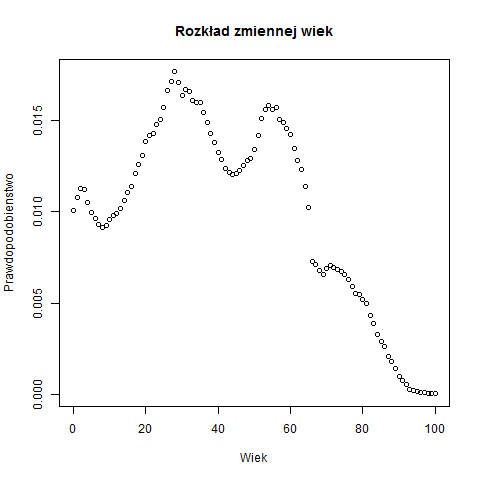
\includegraphics[width=\linewidth]{pictures/wiek.png}
  \caption{Przykładowy rozkład prawdopodobieństwa zmiennej wiek, na podstawie GUS}
  \label{fig:wiek}
\end{figure}

\begin{figure}
  \centering
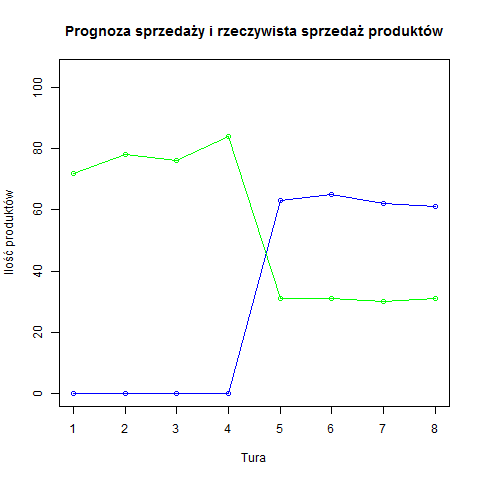
\includegraphics[width=\linewidth]{pictures/wyksztalcenie.png}
  \caption{Przykładowy rozkład prawdopodobieństwa zmiennej wykształcenie ($zielony$ dla mężczyzn, $czerwony$ dla kobiet), na podstawie GUS}
  \label{fig:wyksztalcenie}
\end{figure}


\subsubsection{Przedsiębiorstwo}

Zgodnie z założeniami określonymi w rozdziale 1, symulowane przedsiębiorstwo jest w istocie zbiorem niezależnych agentów, tworzących wspólne sieć neuronową. Zbiór ten należy w modelu do klasy \textit{firma}, przechowującej w podzbiorach instancje klas \textit{fabryka, magazyn, sklep}, jak zaprezentowano na diagramie \ref{firma}. W klasie \textit{firma} znajdują się także funkcje przynależne opisywanemu w strukturze modelu zarządowi, mające na celu koordynację działania przedsiębiorstwa. 

Warto zauważyć, że klasy te mają wiele wspólnych właściwości, z wyjątkami obecnymi w klasie \textit{sklep}, co wynika z konieczności stworzenia funkcji symulujących sprzedaż oraz faktu, że sklepy mają dodatkowe zmienne przechowujące informacje o składzie towaru, klientach odwiedzających sklep w danej jednostce czasu $t$ oraz historii transakcji.  

\begin{tikzpicture} \label{firma}
\begin{class}[text width=7cm]{firma}{-1,0}
\attribute{fabryki : array}
\attribute{magazyny : array}
\attribute{sklepy : array}
\attribute{produkt : array}
\attribute{cena : array}
\operation{klienci\_w\_sklepach(self,swiat,tura)}
\operation{przypisz\_koszty(self,losowe,skala)}

\end{class}
\begin{class}[text width=6cm]{fabryka magazyn}{-5,-7}
\inherit{firma}
\attribute{nazwa : string}
\attribute{lokalizacja : array}
\attribute{oblozenie : integer}
\attribute{koszt : integer}
\attribute{efekt\_skali : integer}
\attribute{symbol : sympy.symbol}
\end{class}
\begin{class}[text width=7cm]{sklep}{2,-7}
\inherit{firma}
\attribute{nazwa : string}
\attribute{lokalizacja : array}
\attribute{oblozenie : integer}
\attribute{koszt : integer}
\attribute{efekt\_skali : integer}
\attribute{symbol:sympy.symbol}

\attribute{klienci : array}
\attribute{klienci\_historycznie : array}
\attribute{sklad : dictionary}
\attribute{sprzedaz : array}
\attribute{przewidywana\_sprzedaz:integer}

\operation{dostawa\_towaru(self, rynek, trasa, ilosc)}
\operation{sprzedaz\_w\_sklepie(self, towar)}
\end{class}
\end{tikzpicture}

\subsubsection{Produkt}

Opierając się na stwierdzeniu \cite{Sagan2011}, który wskazuje na nurtu w dziedzinie modelowania strukturalnego zachowań klientów, które wykorzystywało zmienne marketingowe określające jakość produktu i ilość cech \footnote{Mowa o tzw. nurcie poznawczym albo nurcie teorii przetwarzania informacji - TPI}, zakładamy, że każdy produkt charakteryzuje się cechami wpływające na prawdopodobieństwo jego zakupu przez konsumentów które mogą być wyrażone ilościowo. 

Stąd produkt definiujemy przez zestaw wybranych cech które odróżniają go od produktów konkurencji, a których dziedziną mogą być \textit{factors} \footnote{\textit{factors} rozumiany jako zmienne kategoryczne}, skala ocen $\in R$ bądź zmienne binarne. \footnote{Ich istotność nie jest w tym momencie ważna, ponieważ nawet jeśli w zbiorze znajdzie się cecha mająca mały wpływ na decyzje konsumentów, zostanie ona wyeliminowana na etapie tworzenia modelu bądź drzewa klasyfikacyjnego ze względu brak istotności statystycznej współczynnika}, a klasa \textit{produkt} przechowujące jednowymiarową macierz z cechami produktu $[x_1,x_2,x_3]$

Warto odnotować, że w pracy przyjmujemy, że symulowanym produktem z branży FMCG jest piwo. Ten dość nieelegancki wybór motywowany jest głównie specyfiką produktu, która dobrze pasuje do wymagań stawianych przez model (szczególnie w aspekcie możliwości modelowania decyzji konsumenckich), wśród których są 

	\begin{itemize}
			\item wysoka sprzedaż i idący za tym wysoki obrót towaru w sklepach --- przeciętny polak pije 99 litrów piwa rocznie, co oznacza butelkę kupioną co mniej więcej drugi dzień, \footnote{Dzięki temu możemy założyć, że prawdopodobieństwo zakupu piwa przez klienta to nawet 50\% , a to z kolei gwarantuje odpowiednią ilość iteracji do przeprowadzenia analizy.} 
			\item produkt mają silne marki o ugruntowanych cecach i grupach docelowych --- reklamy piw zazwyczaj podkreślają w jakich okolicznościach i jaka grupa docelowa pije piwo, co powoduje, że występuje wysoka zależność pomiędzy charakterystyką demograficzną klienta a piwem które wybierze, \footnote{Idealnym przykładem jest Redd's, wybierany głównie przez kobiety. Innymi mogą być Grolsch wybierany przez ludzi zamożnych, kiedy Wojak trafia do najgorzej zarabiających}. 
			\item produkty mocno różnią się od siebie cechami --- w przeciwieństwie do mąki, rola jakości, smaku i właściwości piwa odgrywa znaczącą rolę dla klienta. Powoduje to, że piwo smakowe i pszeniczne będą trafiać do dwóch różnych grup klientów.
	\end{itemize}

\subsubsection{Konkurencja}
 
W założeniach przyjmujemy, że konkurencja jest pasywna - tj. nie podejmuje działań ani decyzji w trakcie trwania symulacji. Wynika to z odmiennego celu badania, którym jest analiza działania algorytmów optymalizacyjnych. Nagłe zmiany sprzedaży spowodowane np. obniżeniem ceny przez konkurencję spowodowałyby wątpliwości interpretacyjne i są zbędne. Konkurencja jest za to potrzebna do stworzenia alternatywnych dla symulowanego produktu, o odmiennych cechach i przyciągających klientów o specyficznych charakterystykach, i jej rola ogranicza się do wprowadzenia go na rynek.


\subsubsection{Trasy}

Klasa \textit{trasy} przechowuje wszystkie możliwe kombinacje łańcuchów dostaw, składające się z instacji klas \textit{fabryka}, \textit{magazyn}, \textit{sklep} oraz \textit{scieżek} pomiędzy nimi \footnote{Jako ścieżkę rozumiemy sekwencję punktów z drogami, jakie trzeba przebyć od fabryki do magazynu i od magazynu do skepu}. W przypadku złożonych grafów (czyli sytuacji, kiedy przedsiębiorstwo składa się z wielu jednostek) ilość kombinacji może uniemożliwić swodobne przetwarzanie klasy w pamięci komputera, jednak w takim wypadku można predefiniować zbiór możliwych łańcuchów, spośród których model będzie wybierał najbardziej optymalne trasy. 

Dla każdej z tras, poza informacjami o jednostkach wchodzących w skład przedsiębiorstwa, przechowujemy także informację o \textit{scieżkach} pomiędzy jednostkami. Wynika to z faktu, że transporty pomiędzy poszczególnymi jednostkami także mogą doświadczać efektów skali, \footnote{Przykładowo, pod kątem kosztów na produkt, transport 100 produktów może być bardziej opłacalny niż 10  ze względu na rozłożenie kosztów stałych na większą ilość produktów} a długość ścieżki bezpośrednio wpływa na koszt łańcucha - koszt wzrasta w stosunku do długości ścieżki.

\subsection{Symulowanie decyzji konsumenckich}

Jak wskazano na diagramie \ref{fig:struktura}, podczas wizyty każdego z wirtualnych konsumentów w sklepie symulujemy jego decyzję co do zakupu towaru. W tej części chcemy, aby decyzje konsumentów w modelu jak najbardziej przypominały decyzje klientów w analogicznych sytuacjach w świecie rzeczywistym. \footnote{Warto odnotować, że to nie jest to samo co późniejsze przewidywanie "prognozowanej sprzedaży"} 

Opierając się na \cite{Sagan2011}, wiemy, że jesteśmy w stanie zdefiniować kluczowe cechy konsumenta i cechy marketingowe produktu jako zbiór zmiennych ilościowych. Stąd, w grze eksperymentalnej przeprowadzonej na potrzeby pracy \footnote{Gra dostępna jest pod adresem http://serwer1418288.home.pl/test/piwo/zapisy.php}, poproszono uczestników o stwierdzenie, jakie produkty z dostępnej listy kupi klient o charakterystyce wylosowanej przez program. Po odpowiedzi udzielonej przez gracza, predefiniowane, jakościowe cechy produktu były transponowane na wartości liczbowe \footnote{Na przykład, piwo Grolsh jest drogie, klasy premium i jest lager, stąd otrzyma zapis [5,1,1], a tani smakowy Redd's [3,0,0].} i wraz z ilościowymi cechami klienta oraz zmienną binarną przechowującą informacje \textit{kupił/niekupił} zapisywany na serwerze SQL. 

W programie dane te służą do budowy drzewa klasyfikacyjnego, które - ponieważ dane liczbiowe są w identycznej formie- dla każdej kwerendy o klienta i produkt zwraca prawdopodobieństwo zakupu. Stąd, dla każdego agenta możemy zbudować listę prawdopodobieństw zakupu każdego z towarów dostępnego na rynku, i w ten sposób losowaniem symulować decyzje konsumenckie. To podejście gwarantuje wysokie podobieństwo z wyborami realnych konsumentów ponieważ

	\begin{itemize}
		\item ze względu na wysoką ilość rekordów jest duża szansa, że istnieje zapis o decyzjach klienta o bardzo podobnej charakterystyce
		\item baza danych jest generowania przez decyzje ludzkie, zapewniając wysoką zgodność z analogicznymi wyborami w świecie rzeczywistym
		\item wybór drzewa klasyfikacyjnego  jako metody i wysoki $n$ rekordówpozwala na bardzo pożądany w tej sytuacji \textit{overfit}, który jak opisuje \cite{James2013} powoduje, że dostajemy bardzo dokładne odwzorowanie zbioru uczącego. 
	\end{itemize}

% --- chapter ---------------------------------------------------------
\clearpage
\section{Efekty działania algorytmu optymalizacyjnego}

\subsection{Charakterystyka badanego środowiska}

Sprawdzenie działania modelu odbędzie się w losowo wygenerowanym środowisku, które ze względu na konieczność wielokrotnej replikacji obliczeń w różnych warunkach zostało zapisane i będzie stosowane we wszystkich obliczeniach w niniejszym rozdziale. Środowisko zostało wygenerowane przy założeniach widocznych w tabeli \ref{tab:zalozenia}, a wygenerowane mapy zostały przedstawione na rysunkach \ref{symulowanamapa} i \ref{symulowanaludnosc}.

\begin{table}[hbt] 
  \centering

  \captionsetup{margin=10pt,font=small,labelfont=bf,width=.8\textwidth}

  \caption[Przykład prostej tablicy]{Właściwości generowanego świata. \textit{Źródło:} opracowanie własne.}
  \label{tab:zalozenia}

\vspace*{2ex}
  \begin{tabular}{lccc}
    Właściwość        & Założenie \\ \hline
    Populacja & $10 000$\\
    Wymiar $x$ & $100$\\
    Wymiar $y$ & $100$\\ 
    Udział dróg & $0.3$\\ 
    Gęstość zakrętów dróg & $0.05$\\  
    Udział budynków mieszkalnych & $0.6$\\  
    Udział biurowców \footnote{Biurowce są dla konsumentów miejscem pracy, do których podróżują codziennie} & $0.2$\\  
    Udział przestrzeni komercyjnej \footnote{Przestrzeń komercyjna to miejsca, w którym można założyć sklep, fabrykę bądź magazyn, tak więc razem tworzą zbiór miejsc gdzie przedsiębiorstwo może losowo wygenerować swoją jednostkę}& $0.2$\\  \hline
    Ilość fabryk & 3\\ 
    Ilość magazynów & 3\\ 
    Ilość ilość sklepów & 6\\ 
  \end{tabular}
\end{table}

\begin{figure}[hbt]
  \centering
  \begin{subfigure}[t]{0.45\textwidth}
    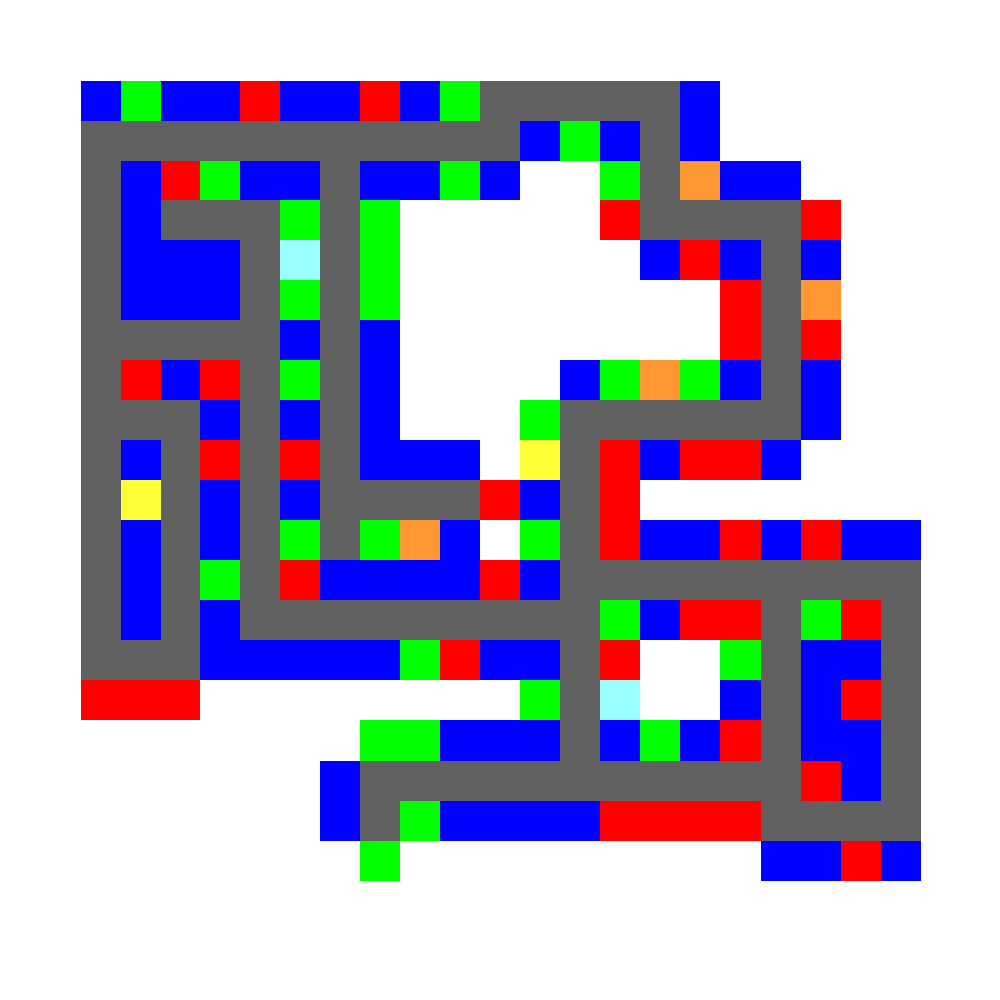
\includegraphics[width=\textwidth]{../mapy/typy.png}
    \caption{Mapa typów lokacji na mapie}
    \label{symulowanamapa}
  \end{subfigure}
  \hfill
  \begin{subfigure}[t]{0.45\textwidth}
    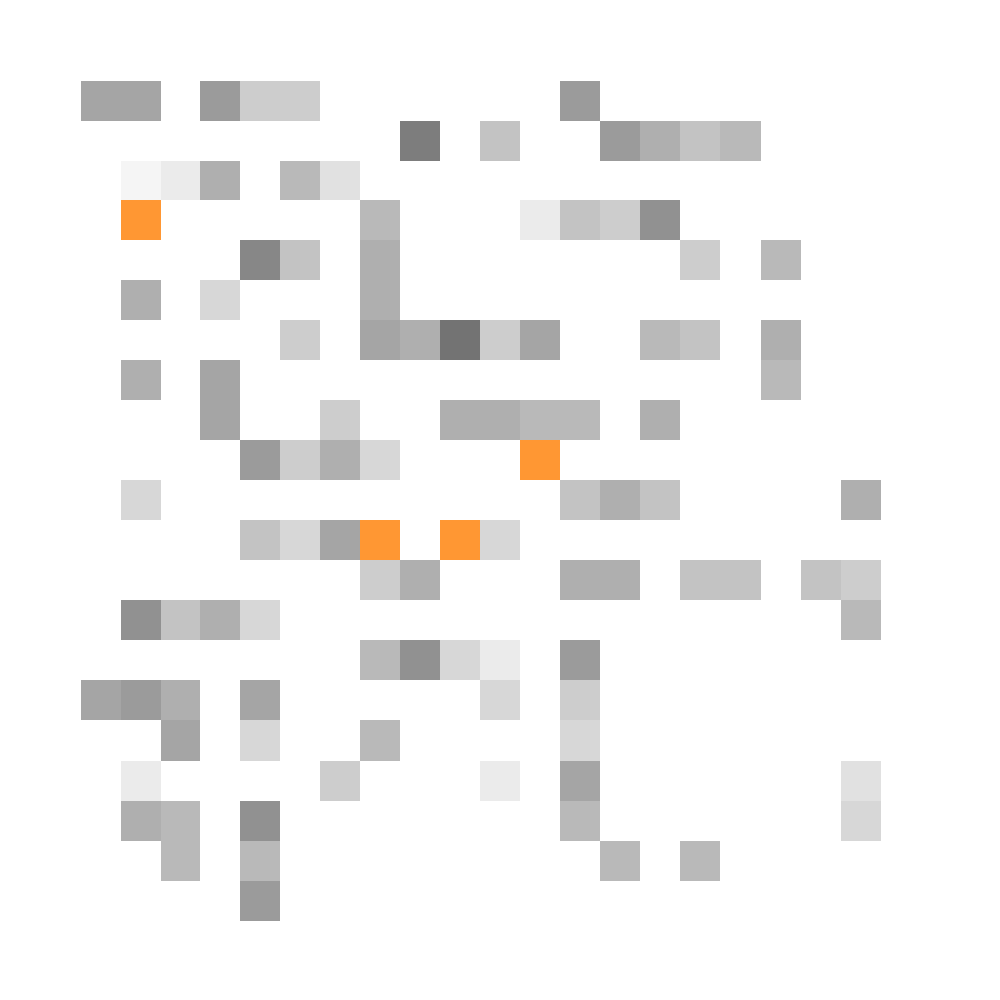
\includegraphics[width=\textwidth]{../mapy/ludnosc.png}
    \caption{Histogram występowania konsumentów na mapie.}
    \label{symulowanaludnosc}
  \end{subfigure}
  
  \captionsetup{margin=10pt,font=small,labelfont=bf,width=.8\textwidth}

  \caption[Krótka nazwa II]{Mapa wygenerowanych macierzy lokalizacji w modelu}\label{fig:xxx}
\end{figure}

\paragraph{Konsumenci}\mbox{}\\
Cechy konsumentów zostały wygenerowane zgodnie z rozkładami zawartymi w Narodowym Spisie Ludności (\cite{GUS2011}) oraz XI Ogólnopolskim Badaniu Wynagrodzień \cite{Sedlak2013} w celu zapewnienia spójności z rzeczywistą strukturą społeczną. Wynikająca z tego histogramy cech klientów zostały zaprezentowane na \ref{ludnosc}. Poza zaprezentowanymi na histogramach danymi demograficznymi agenci posiadają trzy zainteresowania, których rozkład zaprezentowany został w tabeli \ref{tab:zainteresowania}. 

W przeciwieństwie do danych demograficznych, są one niezależne, a każda z nich posiadała identyczną szansę na wylosowanie. Celem tego było wprowadzenie do modelu zmiennych, których nie byłyby skorelowane z innymi, a ponieważ mają wpływ na wybory klientów i nie są zapisywane w historii transakcji, utrudniają przewidywanie sprzedaży.

\begin{table}[hbt] 
  \centering

  \captionsetup{margin=10pt,font=small,labelfont=bf,width=.8\textwidth}

  \caption[Przykład prostej tablicy]{Rozkład zmiennych zainteresowań agentów. \textit{Źródło:} opracowanie własne.}
  \label{tab:zainteresowania}

\vspace*{2ex}
  \begin{tabular}{lccc}
  \hline
 & Ilość \\ 
  \hline
Moda & 1234.00 \\ 
  Gotowanie & 1246.00 \\ 
  Finanse & 1265.00 \\ 
  Kultura & 1213.00 \\ 
  Historia & 1189.00 \\ 
  Koncerty & 1222.00 \\ 
  Motoryzacja & 1219.00 \\ 
  Kosmetyki & 1241.00 \\ 
  Malarstwo & 1260.00 \\ 
  Ogrodnictwo & 1289.00 \\ 
  Gry & 1358.00 \\ 
  Sport & 1255.00 \\ 
  Boks & 1286.00 \\ 
  Fotografia & 1233.00 \\ 
  Kultura alternatywna & 1252.00 \\ 
  Nightlife & 1231.00 \\ 
  Teatr & 1229.00 \\ 
  Ksiazka & 1264.00 \\ 
  Historia polski & 1243.00 \\ 
  Natura & 1233.00 \\ 
  Piwowarstwo & 1202.00 \\ 
  Muzyka klasyczna & 1293.00 \\ 
  Ksiazki & 1233.00 \\ 
   \hline
\end{tabular}
\end{table}

\begin{figure}[hbt]
  \centering
    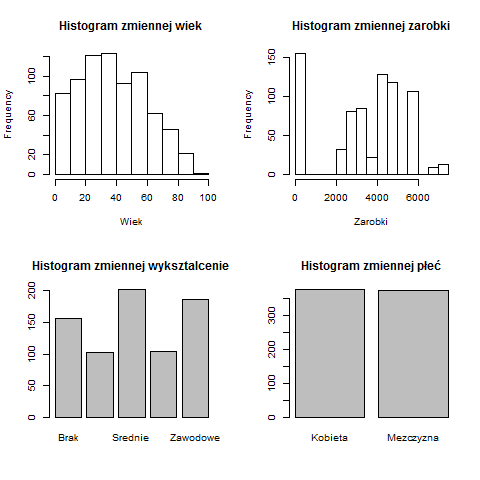
\includegraphics[width=\textwidth]{pictures/ludnosc.png}
  \captionsetup{margin=10pt,font=small,labelfont=bf,width=.8\textwidth}
  \caption[Krótka nazwa X]{Histogramy cech agentów. \textit{Źródło:} opracowanie własne}\label{ludnosc}
\end{figure}

\paragraph{Przedsiębiorstwo}\mbox{}\\
Symulowane przedsiębiorstwo składa się z zaprezentowanej w tabeli \ref{tab:zalozenia} ilości jednostek --- 3 fabryk, 3 magazynów i 6 sklepów, które wspólnie tworzą  $3\choose 1 $ $ \times $ $3\choose 1 $ $ \times $ $6\choose 1 $ = 108 możliwych kombinacji łańcuchów dostaw. Lokacje poszczególnych jednostek zostały zaprezentowane na rysunku \ref{mapafirma}.

\begin{figure}[hbt]
  \centering


    
\includegraphics[width=\textwidth]{../mapy/firma.png}


  \captionsetup{margin=10pt,font=small,labelfont=bf,width=.8\textwidth}

  \caption[Krótka nazwa X]{Mapa z zaznaczonymi jednostkami przedsiębiorstwa. \textit{Źródło:} opracowanie własne}\label{mapafirma}
\end{figure}

\paragraph{Produkty}\mbox{}\\
Zakładamy, że na rynku obecnych jest 7 marek piwa, z których jedno należy do symulowanego przez nas przedsiębiorstwa (produkt o nazwie \textbf{Symulowane}). Każde z piw zdefiniowane jest 7 zmiennymi marketingowymi, z których \textit{cena, smak, opakowanie i marketing} to liczby całkowite w skalie $1-5$, a \textit{premium, budzetowe, lager oraz smakowe} to zmienne binarne. Cechy produktów zaprezentowane zostały w tabeli \ref{tab:produkty}. 

\begin{table}[hbt] 
  \centering

  \captionsetup{margin=10pt,font=small,labelfont=bf,width=.8\textwidth}

  \caption[Przykład prostej tablicy]{Cechy symulowanych produktów. \textit{Źródło:} opracowanie własne.}
  \label{tab:produkty}

\vspace*{2ex}
  \begin{tabular}{rrrrrrrrr}
  \hline
 & Cena & Smak & Opakowanie & P & B & L & S & Marketing \footnote{Zmienne binarne zostały oznaczone literami, P = premium, B = Budżetowe, L=Lager, S=Smakowe}\\ 
  \hline
\textbf{Symulowane} &   1 &   4 &   3 &   1 &   0 &   1 &   0 &   1 \\ 
  Lebskie &   4 &   3 &   4 &   0 &   1 &   1 &   0 &   4 \\ 
  Baltyckie &   1 &   4 &   5 &   1 &   0 &   0 &   1 &   3 \\ 
  Opolskie &   4 &   4 &   4 &   1 &   0 &   1 &   0 &   1 \\ 
  Mocne &   4 &   5 &   4 &   1 &   0 &   0 &   1 &   5 \\ 
  Pyszne &   5 &   1 &   3 &   1 &   0 &   1 &   0 &   2 \\ 
  Babskie &   5 &   4 &   5 &   0 &   0 &   1 &   0 &   3 \\ 
   \hline
\end{tabular}
\end{table} 

\subsection{Przewidywanie decyzji konsumentów}

Przewidywanie decyzji konsumentów odbywa się zgodnie z założeniami przedstawionymi w rozdziale \ref{statistical}. Jednak ponieważ w modelu stosowane jest pewne uproszczenie, polegające na braku symulacji efektów zewnętrznych, a decyzje klientów o przyjściu do sklepu są losowe w ramach zamkniętej puli miejsc, do przewidywania liczby klientów odwiedzających sklep w chwili $t+1$ stosowana jest średnia (ponieważ brak jest zmiennych objaśniających które mogłyby zostać wykorzystane w modelu). Mogłoby to zostać zaaplikowane poprzez wprowadzenie zmiennych losowych typu \textit{pogoda, temperatura, dzień tygodnia}, jednak wprowadzałoby to niepotrzebną złożoność do modelu, a nie wpływa to bezpośrednio na cel badania. 

Jednocześnie, dalsze prognozowanie odbywa się zgodnie z przyjętym podejściem --- tak więc dysponując liczbą klientów w chwili $t+1$ wiemy, ilu konsumentów musimy wylosować na podstawie prawdopodobieństw warunkowych cech zapisanych w historii transakcji. Następne, dla każdego z tak wylosowanych klientów prognozujemy prawdopodobieństwo wybrania każdego z produktów dostępnych w sklepie, otrzymująć jego \textit{decyzję konsumencką}. Estymacja może zostać dokonana metodą regresji logistycznej bądź klasyfikacji \textit{k-means}, w zależności od wyboru użytkownika. Suma decyzji konsumenckich wskazujących symulowany produkt będzie wolumenem sprzedaży w $t+1$. 

Wyniki prognozowanej sprzedaży w stosunku do zrealizowanej sprzedaży w $t+1$ przedstawiony został na wykresie \ref{fig:prognoza}, z kolei porównanie trafności prognoz każdej z metod zostało zaprezentowane w macierzy pomyłek (\textit{confusion matrix}) w tabeli 


\begin{figure}[hbt]
  \centering

  \begin{subfigure}[t]{0.45\textwidth}
    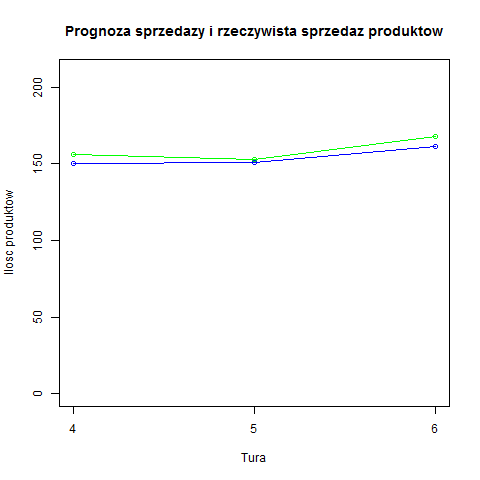
\includegraphics[width=\textwidth]{pictures/prog.png}
  \end{subfigure}

  \captionsetup{margin=10pt,font=small,labelfont=bf,width=.8\textwidth}

  \caption[Krótka nazwa X]{Przykładowy pojedynczy wykres. \textit{Źródło:} opracowanie własne}\label{fig:prognoza}
\end{figure}


\begin{figure}[hbt]
  \centering
  \begin{subfigure}[t]{0.45\textwidth}

\begin{tabular}{rrr}
  \hline
 & 0 & 1 \\ 
  \hline
0 & 892 & 222 \\ 
  1 & 303 & 375 \\ 
   \hline
\end{tabular}
    \caption{Macierz pomyłek dla regresji logistycznej}
    \label{fig:xxxa}
  \end{subfigure}
  \hfill
  \begin{subfigure}[t]{0.45\textwidth}
\begin{tabular}{rrr}
  \hline
 & 0 & 1 \\ 
  \hline
0 & 967 & 147 \\ 
  1 & 498 & 180 \\ 
   \hline
\end{tabular}
    \caption{Macierz pomyłek dla klasyfikacji k-means}
    \label{fig:xxxb}
  \end{subfigure}
  
  \captionsetup{margin=10pt,font=small,labelfont=bf,width=.8\textwidth}

  \caption[Krótka nazwa II]{Przykładowy wykres. Wykresy podpisujemy, a więc ten opis znajduje się pod wykresem. \textit{Źródło:} opracowanie własne}\label{fig:xxx}
\end{figure}



\subsection{Wyniki przedsiębiorstwa przy braku optymalizacji}
\subsection{Optymalizacja przy stałych cenach i braku efektu skali}
\subsection{Optymalizacja przy stałych cenach i istnieniu efektu skali}



% --- chapter ---------------------------------------------------------
\clearpage
\section{Rysunki i tablice}

Zarówno rysunki jak i tablice używają podobnej koncepcji osadzania w dokumencie. Aby osadzić tablicę używa się otoczenia  \verb+table+. Poniżej jest przykład prostej tablicy.

\begin{table}[hbt]
  \centering

  \captionsetup{margin=10pt,font=small,labelfont=bf,width=.8\textwidth}

  \caption[Przykład prostej tablicy]{Przykład prostej tablicy. Ten tekst będzie automatycznie zawijany. \textit{Źródło:} opracowanie własne.}
  \label{tab:exceptional-table}

\vspace*{2ex}

  \begin{tabular}{lccc}
    Name        & property 1 & property 2 & property 3 \\ \hline
    Michael     & 23         & 34         & --         \\
    John        & 34         & --         & 28         \\
    Mr. Niceguy & 123        & 231        & 312        \\ \hline
  \end{tabular}
\end{table}

Tablica~\ref{tab:exceptional-table} jest przykładem bardzo prostej tablicy ale możliwe jest znacznie więcej rzeczy, w razie konieczność służę pomocą.

Aby osadzić rysunek to w pierwszej kolejności trzeba mieć ten rysunek w pliku. W katalogu są dwa przykładowe rysunki. Następujący przykład korzysta z tych rysunków i jest przykładem wykorzystania otoczenia \verb+figure+.

\begin{figure}[hbt]
  \centering

  \begin{subfigure}[t]{0.45\textwidth}
    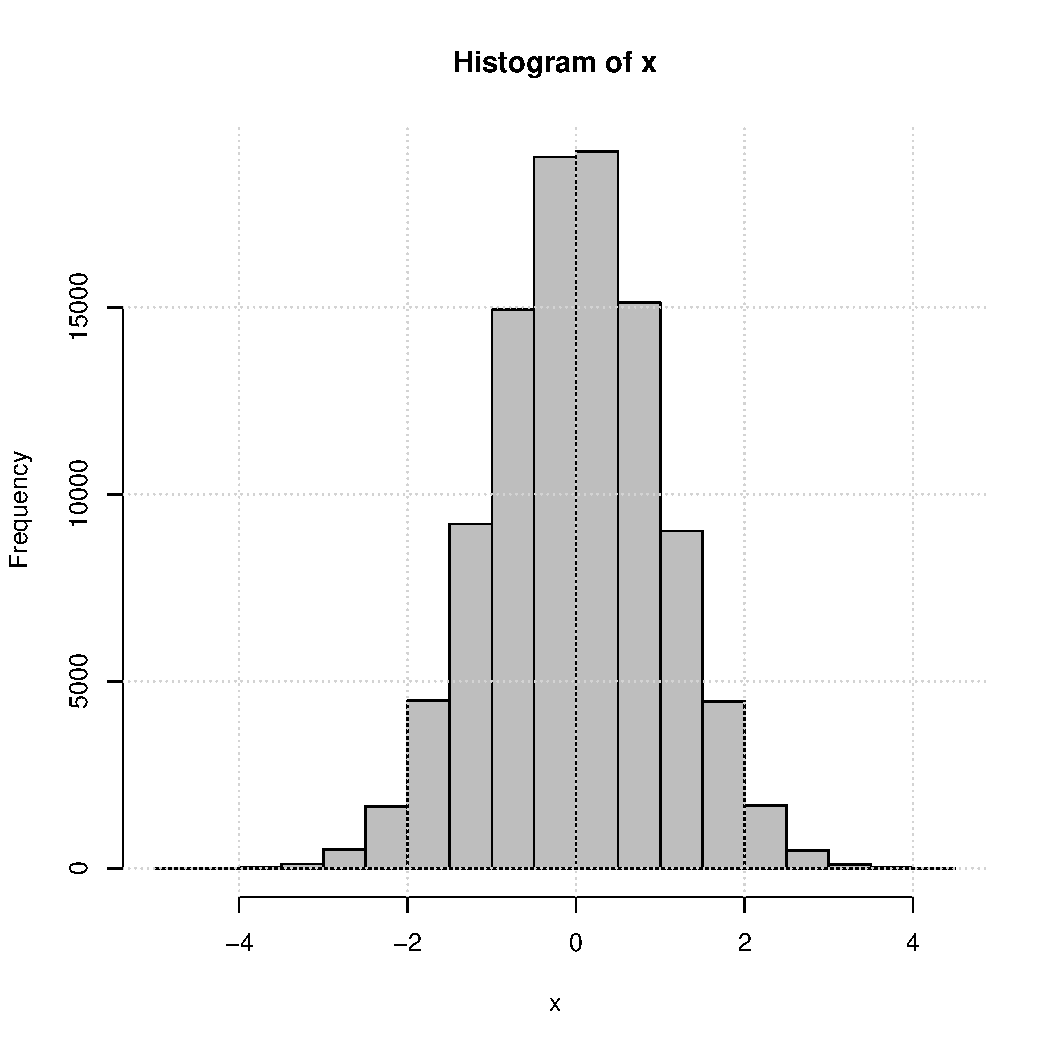
\includegraphics[width=\textwidth]{./figure-1}
  \end{subfigure}

  \captionsetup{margin=10pt,font=small,labelfont=bf,width=.8\textwidth}

  \caption[Krótka nazwa X]{Przykładowy pojedynczy wykres. \textit{Źródło:} opracowanie własne}\label{fig:xxx1}
\end{figure}

\begin{figure}[hbt]
  \centering
  \begin{subfigure}[t]{0.45\textwidth}
    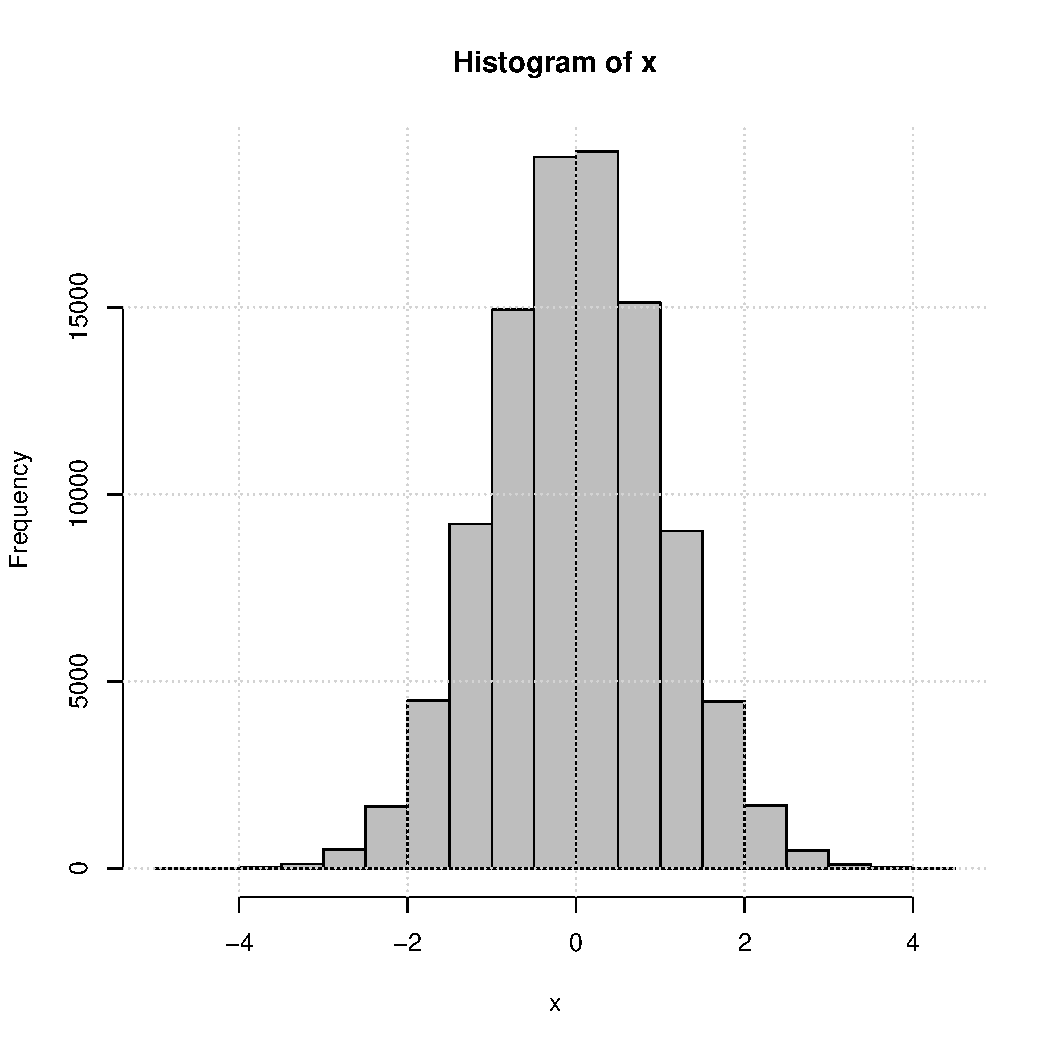
\includegraphics[width=\textwidth]{./figure-1}
    \caption{To jest pierwszy podpis. Ten podpis będzie również zawijany ale będzie to powodowało odpowiednie dopasowanie wysokości.}
    \label{fig:xxxa}
  \end{subfigure}
  \hfill
  \begin{subfigure}[t]{0.45\textwidth}
    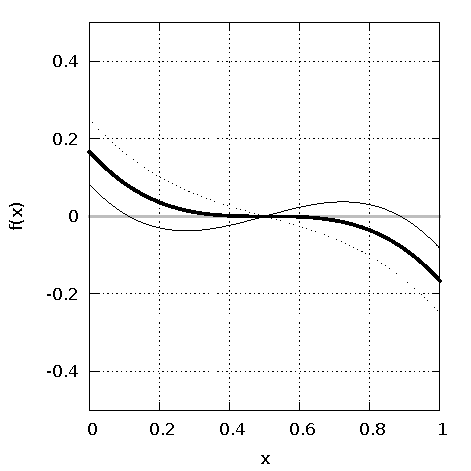
\includegraphics[width=\textwidth]{figure-2}
    \caption{Układ równowag stabilnych}
    \label{fig:xxxb}
  \end{subfigure}
  
  \captionsetup{margin=10pt,font=small,labelfont=bf,width=.8\textwidth}

  \caption[Krótka nazwa II]{Przykładowy wykres. Wykresy podpisujemy, a więc ten opis znajduje się pod wykresem. \textit{Źródło:} opracowanie własne}\label{fig:xxx}
\end{figure}

Odwołanie się do wykresu działa podobnie jak do równania: rysunek~\ref{fig:xxx1}. Możemy również odwoływać się do podwykresów:~\ref{fig:xxxa} lub \ref{fig:xxxb}. Zarówno tablice (tabele) jak i rysunki (wykresy) są automatycznie układane przez \LaTeX{} i nie pozycjinujemy ich sami.


% --- appendices ------------------------------------------------------
\appendix

% ---------------------------------------------------------------------
\clearpage
\section{Dodatek: Ważne rzeczy do dodania}

Tutaj można włożyć długie tablice, kod wykorzystane w pracy lub inne elementy, które nie powinny zakłócać czytania tekstu.


% --- bibliography ----------------------------------------------------
\clearpage
\bibliographystyle{agsm}
\bibliography{refs}

% --- abstract --------------------------------------------------------
\clearpage
\addcontentsline{toc}{section}{Lista tablic}
\listoftables

% --- abstract --------------------------------------------------------
\clearpage
\addcontentsline{toc}{section}{Lista rysunków}
\listoffigures



% --- abstract --------------------------------------------------------
\clearpage
\addcontentsline{toc}{section}{Streszczenie}
\section*{Streszczenie}

Tutaj zamieszczają Państwo streszczenie pracy. Streszczenie powinno być długości około pół strony.


\end{document}

